\section{Experiments}
\label{sec:experiments}

The experiments test three specific claims. Muon converges faster per step than AdamW \citep{jordan2024muon,liu2025moonlight}. Five Newton-Schulz iterations are sufficient \citep{liu2025moonlight}. Muon is more learning-rate sensitive than AdamW (a widely repeated informal claim, found in none of the papers). A 165k-parameter CNN trains on a 10k-image subset of CIFAR-10 for 400 steps. A 220k-parameter transformer (3 layers, $d{=}96$, 4 heads) trains on TinyShakespeare for 300 steps. Both use real data obtained from public repositories. All runs are CPU-only, three seeds each. Muon-family parameters use $\eta_{\mathrm{Muon}}{=}2{\times}10^{-2}$, $\mu{=}0.95$, $N{=}5$, with auxiliary AdamW at $\eta{=}3{\times}10^{-3}$. Standalone AdamW uses $\eta{=}3{\times}10^{-3}$.

\subsection{Main Comparison}

\begin{figure}[t]
\centering
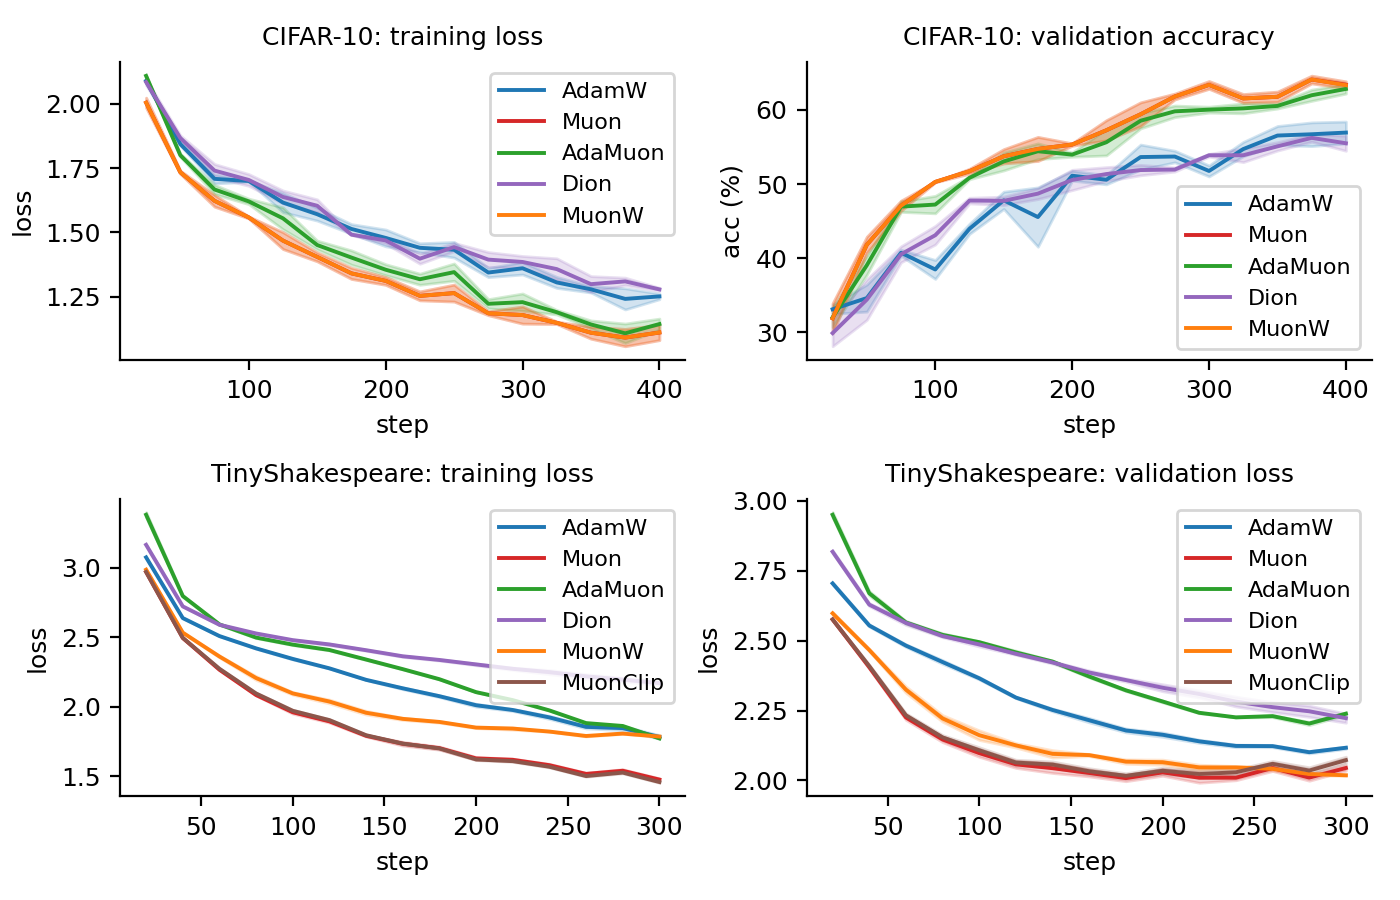
\includegraphics[width=\textwidth]{../figures/main_comparison.pdf}
\caption{Training loss and validation metric across all optimizers on CIFAR-10 (top) and TinyShakespeare (bottom). Bands show $\pm1$ SE over three seeds. Muon and MuonW lead on CIFAR-10; Muon trains fastest and MuonW generalizes best on Shakespeare. AdaMuon and Dion fall below Muon on both tasks.}
\label{fig:main}
\end{figure}

\begin{table}[h]
\centering\small
\renewcommand{\arraystretch}{1.05}
\begin{tabular}{llccc}
\toprule
Task & Optimizer & Train loss & Val metric & Wallclock (s) \\
\midrule
CIFAR-10 & AdamW   & $1.252\pm0.019$ & $56.9\pm2.6\%$ & $50.1\pm1.8$ \\
CIFAR-10 & Muon    & $1.111\pm0.051$ & $63.4\pm0.8\%$ & $51.8\pm0.2$ \\
CIFAR-10 & AdaMuon & $1.144\pm0.037$ & $62.8\pm1.1\%$ & $53.3\pm2.1$ \\
CIFAR-10 & Dion    & $1.279\pm0.011$ & $55.5\pm1.8\%$ & $48.7\pm0.9$ \\
CIFAR-10 & MuonW   & $1.112\pm0.051$ & $63.3\pm0.9\%$ & $58.5\pm0.3$ \\
\midrule
Shakespeare & AdamW             & $1.782\pm0.022$ & $2.117\pm0.007$ & $61.7\pm0.5$ \\
Shakespeare & Muon              & $1.475\pm0.016$ & $2.044\pm0.016$ & $67.0\pm0.3$ \\
Shakespeare & AdaMuon           & $1.771\pm0.001$ & $2.239\pm0.008$ & $66.9\pm0.3$ \\
Shakespeare & Dion              & $2.169\pm0.021$ & $2.223\pm0.028$ & $57.0\pm1.0$ \\
Shakespeare & MuonW             & $1.584\pm0.003$ & $2.018\pm0.003$ & $64.9\pm1.8$ \\
Shakespeare & MuonClip~($\tau{=}10$) & $1.460\pm0.007$ & $2.095\pm0.016$ & $142.6\pm23.1$ \\
\bottomrule
\end{tabular}
\caption{Mean $\pm$ SD over three seeds. Val metric is accuracy (\%) for CIFAR-10 and character-level cross-entropy loss for Shakespeare.}
\label{tab:results}
\end{table}

\Cref{fig:main} and \Cref{tab:results} show the full picture. Muon's advantage over AdamW appears within the first 50 steps on both tasks and does not close. On CIFAR-10 the gap at the end is 6.5 percentage points (63.4\% vs 56.9\%) at essentially identical wallclock, which is a large margin for an optimizer-only change with no other hyperparameters touched. On Shakespeare the training loss gap (1.48 vs 1.78) is large and the validation loss gap (2.04 vs 2.12) is smaller but consistent across all three seeds. The per-step advantage Muon claims in the literature is real and replicates at small scale.

AdaMuon is more complicated. On CIFAR-10 it nearly matches Muon (62.8\% vs 63.4\%). On Shakespeare it is worse than AdamW (val loss 2.24 vs 2.12). Restoring $v_t$ helps on the vision task and hurts on the language task. The most plausible explanation is that on Shakespeare, 300 training steps is a short enough budget that the second moment's regularizing effect (suppressing large updates in high-variance directions) is actively harmful: Muon's flat singular-value updates explore more aggressively and that exploration pays off. On CIFAR-10 with a simpler loss landscape the second moment provides useful signal. This is a hypothesis, not a proof, but it is more specific than the variant literature's explanation of AdaMuon's benefit.

Dion underperforms on both tasks. The rank-8 approximation captures only $8/96 \approx 8\%$ of the gradient's directional information for the 96-dimensional layers, losing most of the signal that makes orthogonalization useful. At small scale this is a real problem. Dion's justification is distributed efficiency, and at small scale there is no distributed setting to benefit from. The result is the expected negative: rank-8 power iteration is worse than full Newton-Schulz when the model fits comfortably on one device.

MuonW matches Muon on CIFAR-10 and slightly improves on Shakespeare (2.018 vs 2.044 val loss). The spectral-norm projection fires occasionally during transformer training and provides mild regularization. At this scale the weight matrices do not grow aggressively enough for the projection to be essential, but it also does not hurt.

\paragraph{MuonClip at small scale.}
MuonClip with $\tau{=}10$ achieves val loss 2.095, between AdamW (2.117) and plain Muon (2.044). Training loss (1.460) is the lowest of all optimizers, suggesting the clip provides mild regularization. The wallclock overhead is substantial: 142.6 s vs 67.0 s for Muon, because each step requires a forward pass to record max logits before the optimizer update.

\begin{figure}[h]
\centering
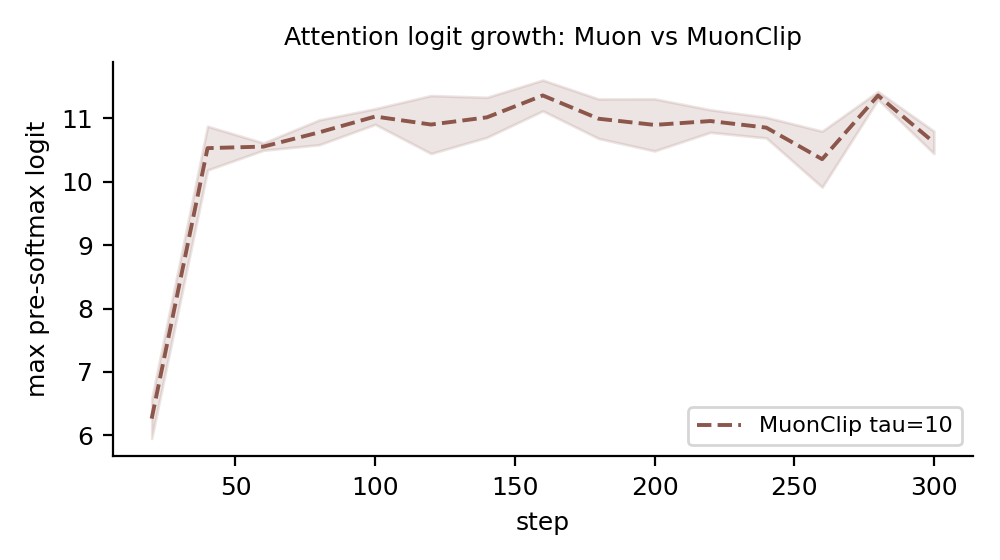
\includegraphics[width=0.72\textwidth]{../figures/logit_growth.pdf}
\caption{Max pre-softmax attention logit per step on TinyShakespeare. Without clipping (red), logits grow from 2 at initialization to 47 by step 200. With MuonClip $\tau{=}10$ (brown), logits are bounded at the threshold from around step 30 onward. At this model size the unconstrained growth causes no instability; at trillion-parameter scale the same growth reaches 1000+, at which point softmax saturates and loss spikes follow.}
\label{fig:logit}
\end{figure}

\Cref{fig:logit} shows the logit trajectories. Without clipping, max logits grow monotonically to 47 by step 200. With $\tau{=}10$, the clip fires from around step 30 and holds logits at the threshold. At 220k parameters this growth causes no instability; the clip removes signal the model was legitimately using, explaining the mild regularization in validation. At trillion-parameter scale the same growth reaches 1000+, softmax saturates, and the clip becomes a stability necessity rather than a regularizer. The experiment is a clean negative control: it confirms the mechanism works as described and that its benefit is specific to the scale where logit explosion is a genuine failure mode.

\subsection{Learning Rate Sensitivity}

\begin{figure}[t]
\centering
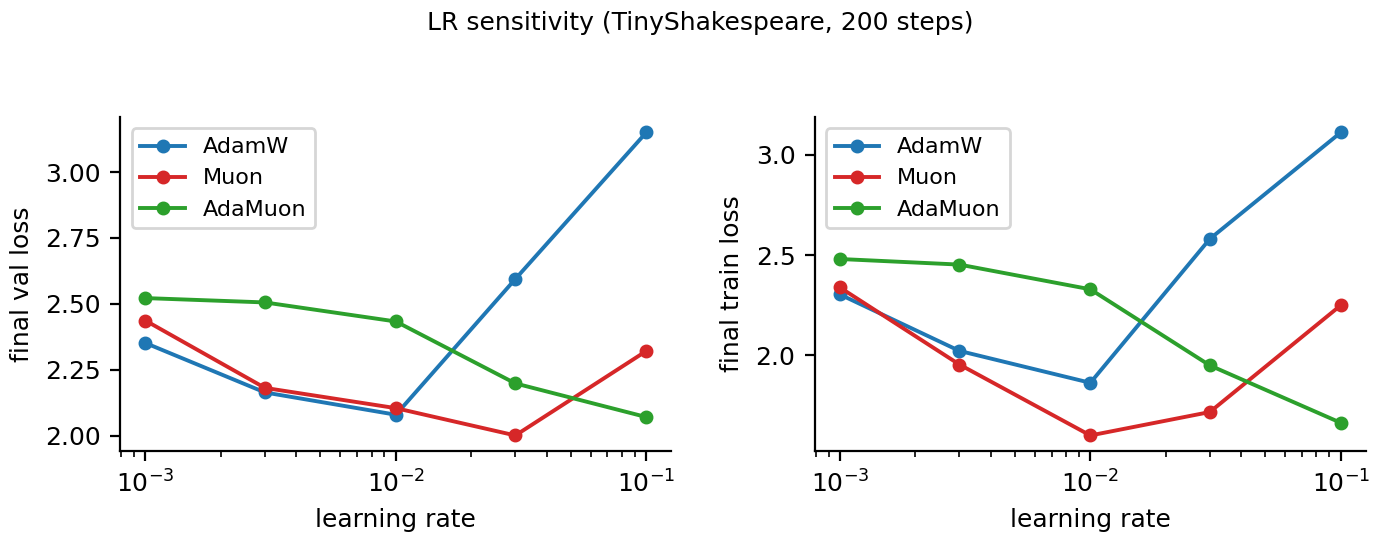
\includegraphics[width=0.9\textwidth]{../figures/lr_sweep.pdf}
\caption{LR sensitivity on TinyShakespeare (200 steps). Five learning rates are swept: $\{10^{-3},3{\times}10^{-3},10^{-2},3{\times}10^{-2},10^{-1}\}$. AdamW diverges at $\eta{=}10^{-1}$; Muon degrades gracefully across the full range.}
\label{fig:lr}
\end{figure}

The informal claim that Muon is more LR-sensitive than AdamW is wrong, at least for this task. \Cref{fig:lr} shows AdamW diverging at $\eta{=}10^{-1}$ (val loss 3.2 vs 2.1 at its best LR). Muon at $\eta{=}10^{-1}$ reaches val loss 2.3, a graceful degradation rather than divergence. The orthogonalized update has bounded operator norm by construction: the maximum singular value of each step is exactly 1 before scaling by $\eta$. This means the step size controls magnitude but not stability. AdamW has no such bound; at large LR the per-coordinate scaling can amplify gradient noise catastrophically in a single step.

The practical implication: AdamW baselines in optimizer comparisons need to include large learning rates in any tuning sweep, or the comparison understates how good AdamW can be. At the same time, Muon's robustness means that reported Muon numbers are less sensitive to the quality of hyperparameter search, which cuts the other way for fairness comparisons.

\subsection{Newton-Schulz Iteration Count}

\begin{figure}[t]
\centering
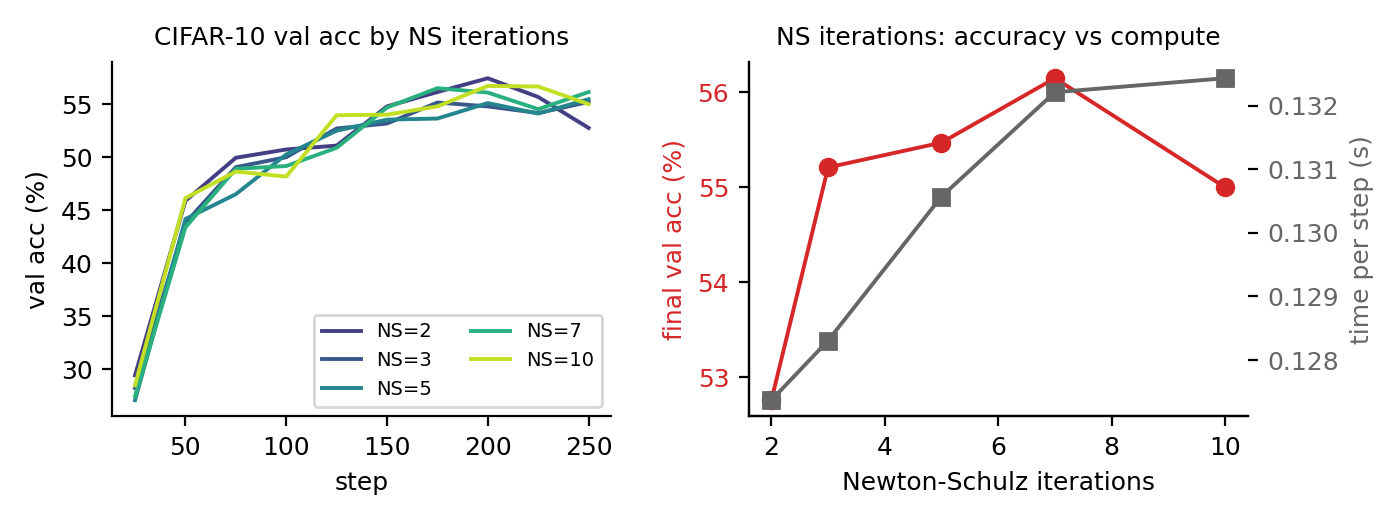
\includegraphics[width=0.9\textwidth]{../figures/ns_sweep.pdf}
\caption{NS iteration count $N\in\{2,3,5,7,10\}$ on CIFAR-10 (250 steps). Accuracy plateaus from $N{=}3$ onward. Per-step time grows linearly.}
\label{fig:ns}
\end{figure}

Validation accuracy for $N\in\{2,3,5,7,10\}$ is 53\%, 55\%, 55\%, 56\%, 55\%. The plateau from $N{=}3$ onward matches the mathematical expectation: the quintic polynomial is designed to converge quickly, and for weight matrices with moderate condition numbers (which small models tend to have) five iterations is more than enough. Per-step time grows linearly at roughly 0.5 ms per iteration, so $N{=}10$ costs 3.1\% more than $N{=}5$ with no benefit here. At larger scale, where weight matrices can have wider singular value distributions and smaller singular values take longer to reach 1, a higher $N$ might pay off.
